\documentclass[a4paper,11pt]{article}
\usepackage[polish]{babel}
\usepackage[utf8]{inputenc}
\usepackage[T1]{fontenc}
\usepackage{times}
\usepackage{graphicx}
\usepackage{anysize}
\usepackage{amsmath}
\usepackage{color}
\usepackage{listings}
\lstloadlanguages{C++}

%\marginsize{left}{right}{top}{bottom}
\marginsize{2.5cm}{2.5cm}{2.5cm}{2.5cm}

\definecolor{darkred}{rgb}{0.9,0,0}
\definecolor{grey}{rgb}{0.4,0.4,0.4}
\definecolor{orange}{rgb}{1,0.6,0.05}
\definecolor{darkgreen}{rgb}{0.2,0.5,0.05}


\begin{document}

\section{Podstawy stosowania pakietu listings}

\lstset{language=C++,
basicstyle=\ttfamily\small,
keywordstyle=\color{darkgreen}\ttfamily\bfseries\small,
stringstyle=\color{red}\ttfamily\small,
commentstyle=\color{grey}\ttfamily\small,
numbers=left,
numberstyle=\color{darkred}\ttfamily\scriptsize,
identifierstyle=\color{blue}\ttfamily\small,
showstringspaces=false,
morekeywords={
}}

W trywialnym przypadku program z języku C++ może składać się tylko z jednego pliku i jednej funkcji. \emph{Funkcja} jest wydzieloną częścią programu, realizującą pewne zadanie.  Kompletny program musi \mbox{zawierać} funkcję o nazwie \emph{main} od której rozpoczyna się wykonanie programu. Do programu można dołączać pliki zawierające nagłówki (opis) funkcji zdefiniowanych w~innych plikach lub funkcji systemowych (dyrektywa \verb!include!).

\vspace{15mm}

\begin{verbatim}
#include <iostream>

int main()
{
  std::cout << "C++\n";
}
\end{verbatim}


\begin{lstlisting}
#include <iostream>

int main()
{
  std::cout << "C++\n";
}
\end{lstlisting}

%--------------------------------------------------------------------------------

Komentarz w C++, to dowolnej długości tekst ograniczony znakami \lstinline!/*! i \lstinline!*/! lub tekst od znaku \lstinline!//! do końca linii.

\begin{lstlisting}[numbers=none]
int main() {  /* Ten program nic nie robi. */ }
\end{lstlisting}

\lstset{language=Ada,
basicstyle=\ttfamily\small,
commentstyle=\ttfamily\small,
keywordstyle=\bfseries\small,
stringstyle=\ttfamily\small,
showstringspaces=false,
identifierstyle=\ttfamily\small,
numbers=right,
morekeywords={
}}

Ada należy do języków rodziny Algol/Pascal, programy napisane w~Adzie są czytelne i~stosunkowo łatwe do analizy.

\begin{lstlisting}
with Text_IO, Ada.Integer_Text_IO; 
use  Text_IO, Ada.Integer_Text_IO; 

procedure Silnia is 
  n, s, i : Integer := 1;

begin  
  Get(n);  

  while i < n loop
    i := i + 1;
    s := s * i;
  end loop;  

  Put("Silnia: "); 
  Put(s, 0);
end;
\end{lstlisting}

\newpage

\section{Definiowanie własnego języka programowania}


\lstdefinelanguage{Alvis}
{
keywords={agent,in,out,delay,jump,exec,alt,data,type,critical,start,exit,far,loop,
if,else,elseif,select,cli,sti,proc,elseif,every,environment,null},
ndkeywords={Char,Bool,Int,Double,String,rem,sqrt,head,tail,signal,durable,queue},
sensitive=true,
morecomment=[l]{--},
morecomment=[s]{/*}{*/},
morestring=[b]",
}

\lstset{language=Alvis,
basicstyle=\ttfamily\small,
commentstyle=\ttfamily\small,
classoffset=0,
keywordstyle=\color{darkred}\ttfamily\bfseries\small,
classoffset=1,
keywordstyle=\color{orange}\ttfamily\small,
classoffset=0,
stringstyle=\ttfamily\small,
commentstyle=\color{blue}\ttfamily\itshape\small,
numbers=left,
numberstyle=\color{blue}\ttfamily\scriptsize,
identifierstyle=\ttfamily\small,
showstringspaces=false,
morekeywords={
}} 

\emph{Język opisu dynamiki} (\emph{Alvis Code Language}, w~skrócie AlvisCD, służy do definiowania zachowania indywidualnych agentów. Występujące w~nim instrukcje są wzorowane na wybranych operatorach algebry CCS, które w~XCCS stosowane były w~warstwie algebraicznej. W~przeciwieństwie do języków modelowania CCS i~XCCS, które skupiają się głównie na opisie komunikacji, marginalizując kwestie związane z~manipulowaniem wartościami parametrów, język Alvis pozwala na wygodne modyfikacje wartości parametrów agenta, niezależne od instrukcji dotyczących komunikacji. 

\begin{lstlisting}
environment {
  in wakeup [] (map (60000*) [1..]) durable;
  in off [] (map (1000*) [1..]) signal;
  out warning [0,1,2] [];
  out brake [] [];  
}

agent ATS {
  loop {                             -- 1
    in wakeup;                       -- 2
    out warning 1;                   -- 3
    select {                         -- 4
      alt (ready [in(off)]) {
        in off;                      -- 5
        out warning 0;               -- 6
      }
      alt(delay 6000) {
        out warning 2;               -- 7
        select {                     -- 8
          alt (ready [in(off)]) {
            in off;                  -- 9
            out warning 0;           -- 10
          }
          alt (delay 3000) {
            out brake;               -- 11
            exit;                    -- 12
          } 
        } 
      } 
    } 
  } 
}
\end{lstlisting}

\textbf{UWAGA:} Pakiet listings pamięta poprzednie ustawienia, jeśli ich nie nadpiszemy, tzn. jeżeli dla poprzedniej specyfikacji ustawiliśmy wyświetlanie numerów linii po prawej stronie, a w kolejnej specyfikacji nic o liczbach nie piszemy, to nadal będą wyświetlane po prawej stronie.

\newpage

\section{Podpisy, odwołania i ramki}

\begin{lstlisting}[caption=Przykład agenta pasywnego,
captionpos=b, label=src:passive]
agent Buffer {
  i :: Int = 0;
  proc pop  { out pop i; }
  proc push { in  push i; }
}
\end{lstlisting}

Agenty pasywne są stosowane do opisu współdzielonych zasobów. Przykładową implementację jednokomórkowego bufora pokazano na listingu~\ref{src:passive}. 


\begin{lstlisting}[caption=Przykład agenta pasywnego, captionpos=b,
label=src:passive2, firstnumber=12,frame=single]
agent Buffer {
  i :: Int = 0;
  proc pop  { out pop i; }
  proc push { in  push i; }
}
\end{lstlisting}

Na listingu~\ref{src:passive2} ciągle rozważamy ten sam przykład, ale w ramce ;)


\begin{lstlisting}[caption=Przykład agenta pasywnego, captionpos=t,
label=src:passive3, frame=tbLR]
agent Buffer {
  i :: Int = 0;
  proc pop  { out pop i; }
  proc push { in  push i; }
}
\end{lstlisting}


\begin{lstlisting}[caption=Przykład agenta pasywnego, captionpos=t,
label=src:passive4, frame=TB]
agent Buffer {
  i :: Int = 0;
  proc pop  { out pop i; }
  proc push { in  push i; }
}
\end{lstlisting}



\begin{lstlisting}[caption=Przykład agenta pasywnego, captionpos=t,
label=src:passive5, frame=LBtr, frameround=tftf]
agent Buffer {
  i :: Int = 0;
  proc pop  { out pop i; }
  proc push { in  push i; }
}
\end{lstlisting}

Narożniki podajemy od prawego {\color{blue}górnego począwszy zgodnie z} ruchem wskazówek zegara. Należy podać dokładnie 4 litery, \emph{t} oznacza zaokrąglony narożnik, a \emph{f} prosty.

Można połączyć grafikę z kodem w ramach jednego środowiska \emph{figure}, tak jak pokazano na rysunku~\ref{fig:queue}.

\begin{figure}[!ht]
\centerline{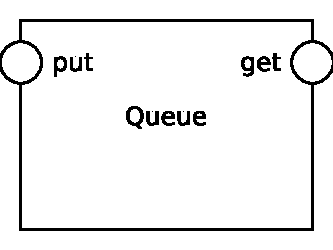
\includegraphics[scale=0.65]{queue}}
\begin{lstlisting}[aboveskip=4mm]
agent Queue {
  q :: [Int] = [];
  n :: Int = 0;

  proc put {
    critical {Przyklad agenta pasywnego
      in put n;
      q = q ++ [n]; } 
  }
  proc get (q /= []) {
    critical {
      n = head q;
      q = tail q;
      out get n; } 
  }
}
\end{lstlisting}
\caption{Agent \emph{Queue}}
\label{fig:queue}
\end{figure}







\end{document}
